\documentclass[aspectratio=169]{beamer}

\usetheme{Madrid}
\setbeamertemplate{navigation symbols}{}
\setbeamertemplate{footline}[frame number]

\usepackage[utf8]{inputenc}
\usepackage{graphicx}
\usepackage{booktabs}
\usepackage{amsmath}

\definecolor{myGreen}{HTML}{009865}
\usecolortheme[named=myGreen]{structure}

\title[Unsupervised KIRC Classification]{Unsupervised Classification of Tumor vs.\ Normal \\ in TCGA-KIRC DNA Methylation Data}
\subtitle{Pseudo-Labeling via Dimensionality Reduction and Clustering}
\author{}
\date{}

\begin{document}

% ---------------------------------------------------------------
\begin{frame}
  \titlepage
\end{frame}

% ---------------------------------------------------------------
\begin{frame}{Motivation}
  \begin{itemize}
    \item \textbf{Goal:} classify tumor vs.\ normal kidney tissue (TCGA-KIRC) from DNA methylation --- \textbf{no ground-truth labels used for training}
    \item \textbf{Pipeline:} dimensionality reduction $\rightarrow$ clustering $\rightarrow$ pseudo-labels $\rightarrow$ classifier
    \item \textbf{Key question:} how good must pseudo-labels be before a classifier trained on them matches one trained on ground truth?
    \item Ground truth is used only to \emph{evaluate} the pipeline --- never to train it
  \end{itemize}
\end{frame}

% ---------------------------------------------------------------
\begin{frame}{Data \& Pipeline Overview}
  \begin{itemize}
    \item TCGA-KIRC Illumina 450K methylation array, 371{,}082 probes after QC
    \item \textbf{Patient-grouped} train/holdout split (285 / 198 samples) --- no patient's tumor/normal pair crosses the split
  \end{itemize}
  \vspace{0.3cm}
  \begin{center}
  \begin{tabular}{ccccc}
    Raw methylation & $\rightarrow$ & Dim.\ reduction & $\rightarrow$ & Clustering \\
    (371k probes)   &               & (PCA vs.\ UMAP) &               & (KMeans / Hierarchical / GMM) \\
  \end{tabular}
  \vspace{0.2cm}

  $\downarrow$

  \vspace{0.2cm}
  Pseudo-labels $\rightarrow$ Classifier (SVM / Random Forest) $\rightarrow$ Evaluate vs.\ ground truth
  \end{center}
\end{frame}

% ---------------------------------------------------------------
\begin{frame}{Methodological Safeguards}
  \begin{itemize}
    \item Patient-grouped splitting everywhere: train/holdout \emph{and} 5-fold cross-validation
    \item Best clustering configuration selected \textbf{automatically} by ARI vs.\ ground truth --- no hand-picked columns
    \item Deployment pool restricted to algorithms that support \texttt{predict()} on new data (excludes hierarchical clustering)
    \item Cross-validation directly re-validates the \emph{same} deployed configuration, not just a related one
    \item Holdout checks catch overfitting that training-ARI alone misses (e.g.\ a full-covariance GMM that fit training data well but collapsed on holdout)
  \end{itemize}
\end{frame}

% ---------------------------------------------------------------
\begin{frame}{Result 1: PCA vs.\ UMAP for Pseudo-Labeling}
  \begin{columns}
    \column{0.55\textwidth}
    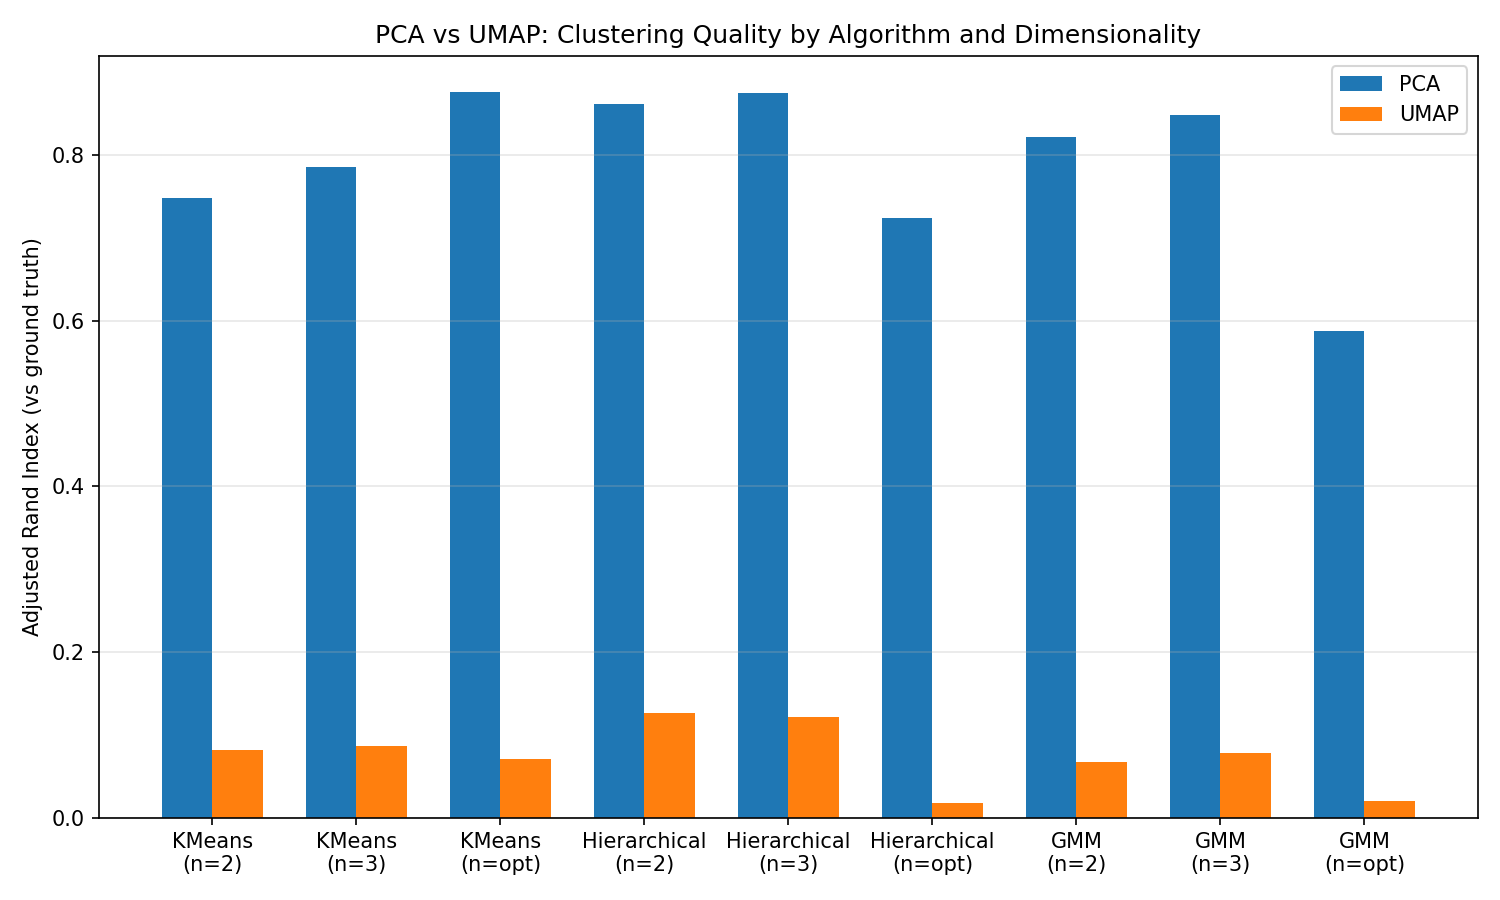
\includegraphics[width=\textwidth]{figures/pca_vs_umap_comparison.png}
    \column{0.45\textwidth}
    \begin{itemize}
      \item PCA beats UMAP in \textbf{every} algorithm $\times$ dimensionality tested
      \item Mean ARI: \textbf{0.79 (PCA)} vs.\ \textbf{0.07 (UMAP)}
      \item Tumor/normal signal is a broad, global shift --- exactly what PCA captures; UMAP optimizes for local structure instead
    \end{itemize}
  \end{columns}
\end{frame}

% ---------------------------------------------------------------
\begin{frame}{Result 2: Clustering Algorithm Search (PCA space)}
  \centering
  \begin{tabular}{lccc}
    \toprule
    Algorithm & $n$ = 2 & $n$ = 3 & $n$ = opt.\ \\
    \midrule
    KMeans        & 0.749 & 0.786 & \textbf{0.876} \\
    Hierarchical  & 0.862 & \textbf{0.876} & 0.724 \\
    GMM           & 0.822 & \textbf{0.848} & 0.588 \\
    \bottomrule
  \end{tabular}
  \vspace{0.4cm}
  \begin{itemize}
    \item ARI against ground truth, 9 configurations compared
    \item \textbf{KMeans, $n=112$} selected automatically as the best deployable configuration
  \end{itemize}
\end{frame}

% ---------------------------------------------------------------
\begin{frame}{Result 3: Pseudo-Label vs.\ Ground-Truth Classifiers}
  \begin{columns}
    \column{0.55\textwidth}
    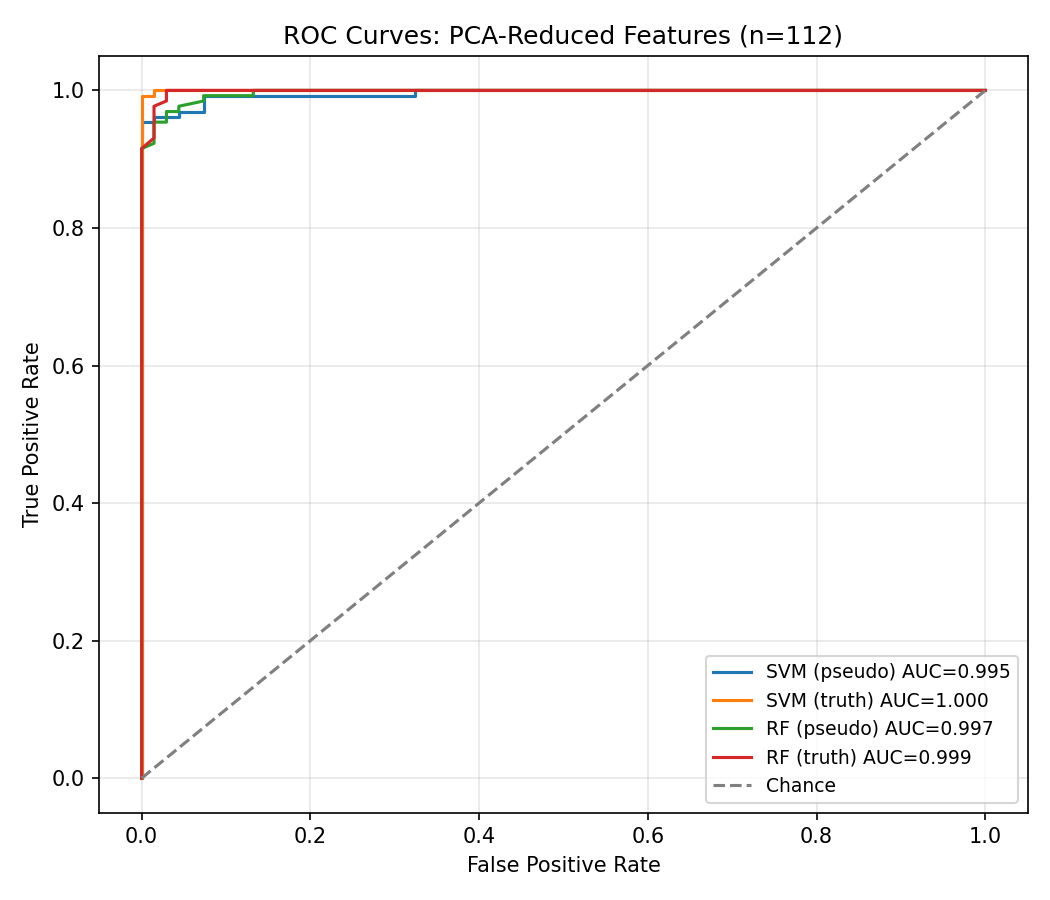
\includegraphics[width=\textwidth]{figures/roc_curves_pca_validation.png}
    \column{0.45\textwidth}
    \begin{itemize}
      \item Classifiers trained on pseudo-labels nearly match classifiers trained on ground truth
      \item SVM: 0.995 (pseudo) vs.\ 1.000 (truth)
      \item RF: 0.997 (pseudo) vs.\ 0.999 (truth)
      \item Gap $<$ 0.005 AUC in both cases
    \end{itemize}
  \end{columns}
\end{frame}

% ---------------------------------------------------------------
\begin{frame}{Result 4: Robustness --- 5-Fold Patient-Grouped CV}
  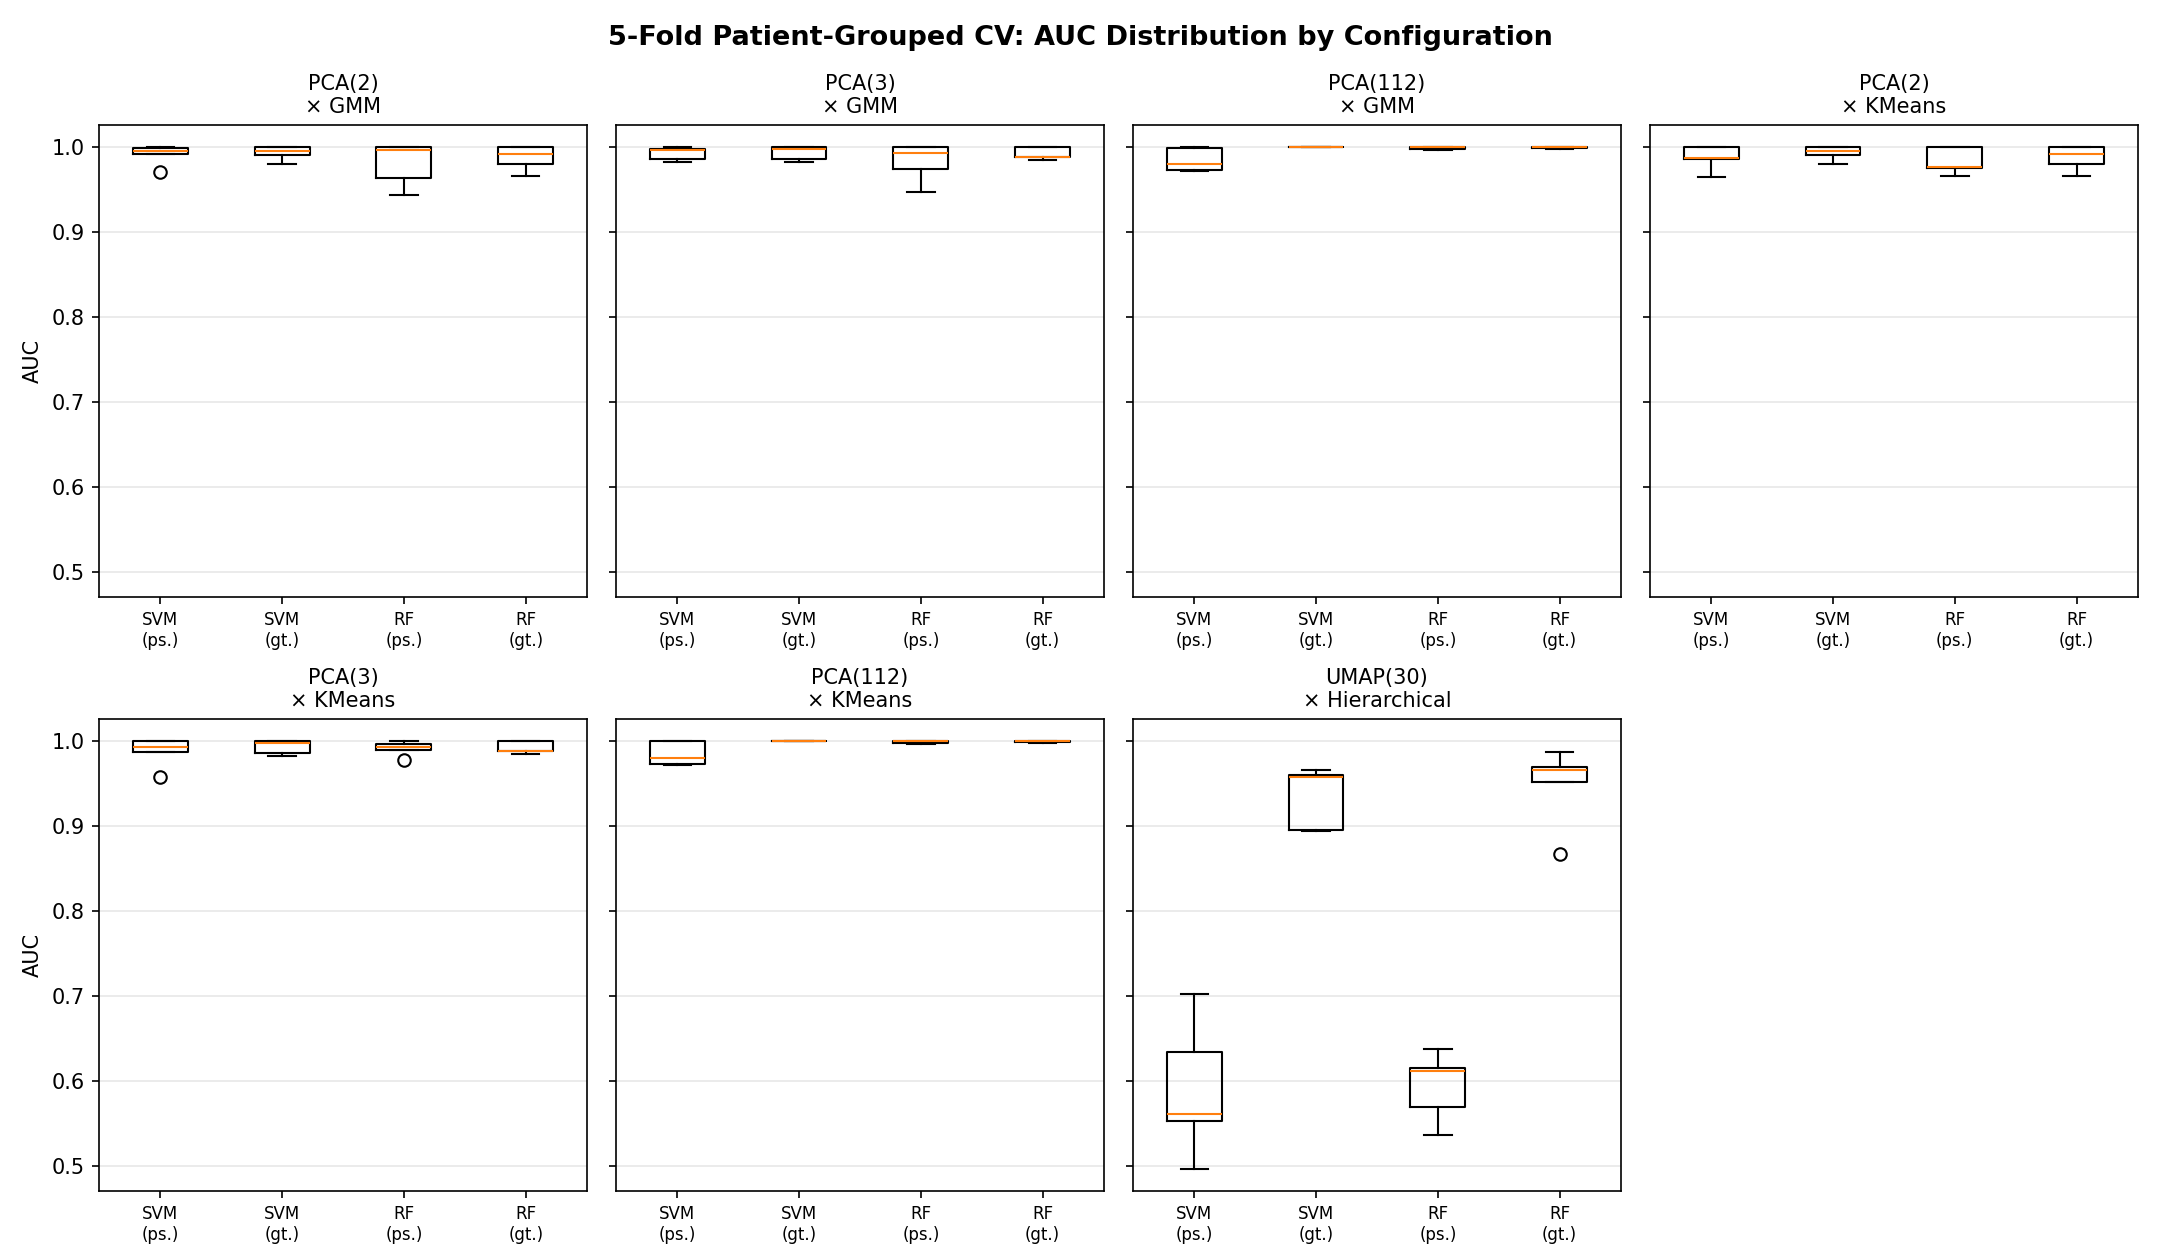
\includegraphics[width=0.95\textwidth]{figures/cv_auc_boxplot.png}
  \begin{itemize}
    \item Six PCA$\times$\{GMM, KMeans\} configurations: AUC $\geq$ 0.98, low variance across folds
    \item \textbf{The deployed model reproduces its own result}: PCA(112)$\times$KMeans CV ARI = 0.850, vs.\ 0.876 (single split) and 0.825 (holdout)
    \item Deliberately poor UMAP(30)$\times$Hierarchical arm (rightmost): consistently low, showing what failure looks like
  \end{itemize}
\end{frame}

% ---------------------------------------------------------------
\begin{frame}{Central Hypothesis: Clustering Quality Predicts Classifier Trustworthiness}
  \begin{columns}
    \column{0.55\textwidth}
    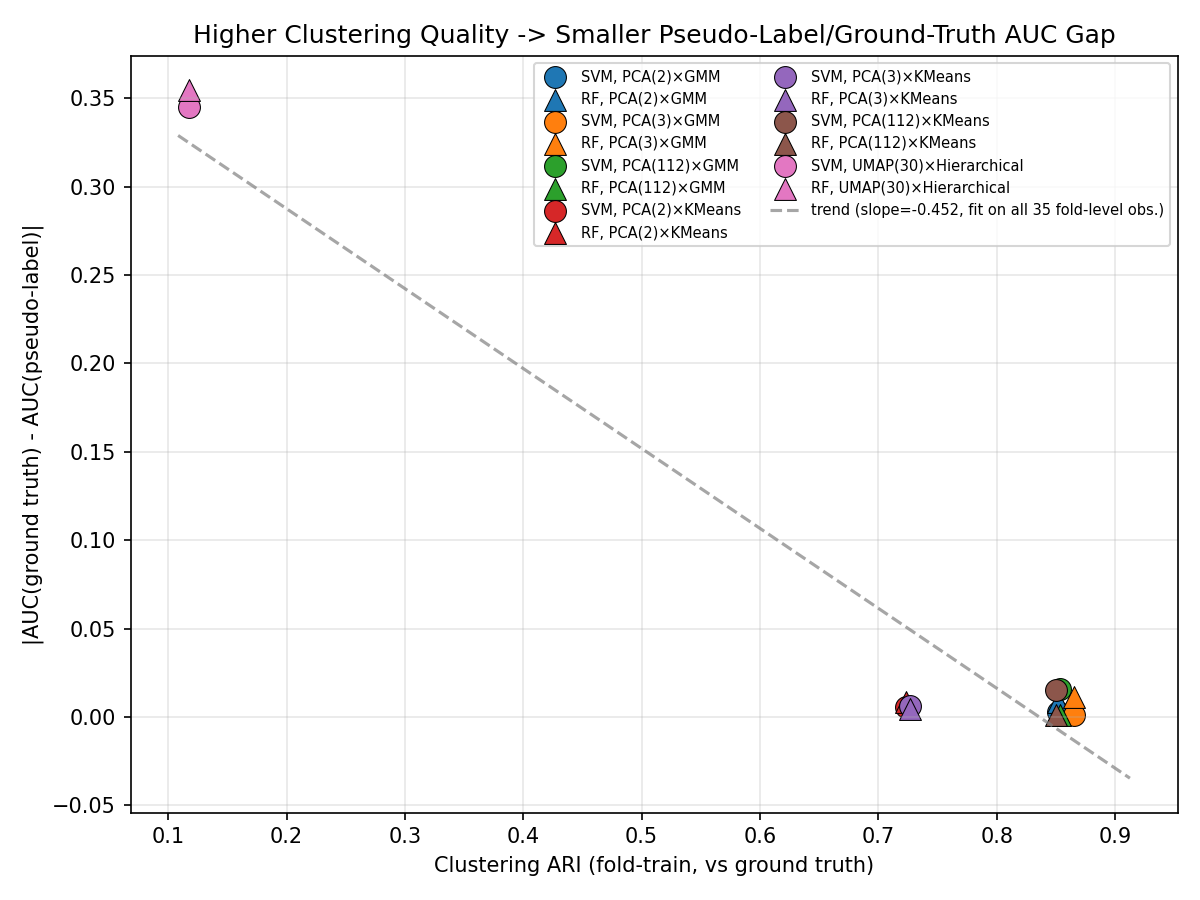
\includegraphics[width=\textwidth]{figures/cv_ari_vs_auc_gap_scatter.png}
    \column{0.45\textwidth}
    \begin{itemize}
      \item \textbf{Claim:} higher clustering ARI $\rightarrow$ smaller gap between pseudo-label and ground-truth classifier AUC
      \item Confirmed across 35 fold$\times$configuration observations, spanning near-zero to near-perfect ARI
      \item Correlation: \textbf{$r=-0.93$ (SVM)}, \textbf{$r=-0.94$ (RF)}
      \item ARI can \emph{predict} classifier trustworthiness before ever checking ground truth on new data
    \end{itemize}
  \end{columns}
\end{frame}

% ---------------------------------------------------------------
\begin{frame}{But: Label-Free Metrics Cannot Replace ARI}
  \begin{itemize}
    \item ARI itself needs ground truth. Can \emph{fully} label-free metrics (silhouette, Davies--Bouldin) do the same job?
    \item \textbf{Tested directly --- answer is no:} correlation with ARI is statistically indistinguishable from zero
    \begin{itemize}
      \item Silhouette vs.\ ARI: $r=0.18$ ($p=0.60$)
      \item Davies--Bouldin vs.\ ARI: $r=-0.17$ ($p=0.63$)
    \end{itemize}
    \item Why: both metrics degrade as dimensionality increases (curse of dimensionality); ARI does not
    \item \textbf{Practical takeaway:} trusting an unsupervised pipeline still requires \emph{some} labeled reference data --- not zero
  \end{itemize}
\end{frame}

% ---------------------------------------------------------------
\begin{frame}{Generalization to Held-Out KIRC Samples}
  \begin{itemize}
    \item Fitted pipeline (PCA + KMeans) applied to a held-out, patient-disjoint split of the \textbf{same} TCGA-KIRC cohort:
    \begin{itemize}
      \item Training ARI: 0.876 \quad$\rightarrow$\quad Holdout ARI: 0.825
    \end{itemize}
    \item Confirmed again under 5-fold CV (ARI $=0.850\pm0.027$) --- little degradation, same result three ways
    \item \textbf{This study can serve as the reference cohort} for future KIRC methylation datasets on the same platform
    \item \textbf{Scope:} tuned to KIRC's epigenetic landscape --- not claimed optimal for other cancer types
  \end{itemize}
\end{frame}

% ---------------------------------------------------------------
\begin{frame}{Comparison to Published Benchmarks}
  \begin{itemize}
    \item Our AUC ($\sim$0.99--1.00) is consistent with, not an outlier from, the literature:
    \item Ding et al.\ (2019, \emph{Epigenetics}): 7 CpG sites separate tumor from normal across 12 TCGA cancers (KIRC included), \textbf{AUC $>$ 0.99}
    \item Liu et al.\ (2019, \emph{Genes}): pan-cancer deep learning, \textbf{AUC 0.993--0.995}
    \item KIRC-specific literature has moved on to the \emph{harder} problem of prognosis (AUC $\sim$0.75--0.82) --- tumor/normal is already near-solved
    \item \textbf{Our contribution:} reaching that same near-ceiling performance \textbf{without supervision}
  \end{itemize}
\end{frame}

% ---------------------------------------------------------------
\begin{frame}{Limitations \& Future Work}
  \begin{itemize}
    \item No external (independent-cohort) validation yet --- holdout is same-cohort, same platform
    \item Pipeline tuned specifically for KIRC; other cancers may favor different configurations
    \item ARI-vs-gap relationship used one deliberately poor clusterer; a broader sweep would strengthen the estimate further
    \item Next steps: external KIRC cohort validation; extend pseudo-labeling to multi-class subtyping
  \end{itemize}
\end{frame}

% ---------------------------------------------------------------
\begin{frame}{Take-Home Messages}
  \begin{enumerate}
    \item \textbf{PCA} clearly beats UMAP for KIRC methylation pseudo-labeling (mean ARI 0.79 vs.\ 0.07)
    \item Pseudo-labels are \textbf{nearly interchangeable with ground truth} for training a classifier (AUC gap $<$ 0.005)
    \item \textbf{Clustering quality (ARI) predicts classifier trustworthiness} ($r=-0.93$ to $-0.94$) --- but this needs some reference labels; fully label-free metrics do not work
    \item The pipeline generalizes within the KIRC cohort and is consistent with published pan-cancer benchmarks
  \end{enumerate}
\end{frame}

% ---------------------------------------------------------------
\begin{frame}
  \centering
  \Large Thank you \\[0.3cm]
  \normalsize Questions? \\[0.5cm]
  {\small Code: \url{https://github.com/ich-bin-tyrone/epi-clusters}}
\end{frame}

\end{document}
